\documentclass{report}
\usepackage{ucs}
\usepackage[utf8x]{inputenc}
\usepackage[T1]{fontenc}
\usepackage[french]{babel}
\usepackage{graphicx}
\usepackage{verbatim} %Pour insérer du code dans le document
\usepackage{listings}
\usepackage{color}
\usepackage{titling}
\usepackage{mwe}
\usepackage{amsmath,amsfonts}
\usepackage{amssymb}
\usepackage{hyperref}
\usepackage[export]{adjustbox}
\usepackage[final]{pdfpages}

\include{java_latex}

\begin{document}

\include{presentation}
\hypersetup{hidelinks}

\tableofcontents

\chapter{Introduction}

Ce rapport a pour ambition de présenter notre projet effectué dans le cadre de l'UE Réseau et Projet
de Programmation 2. Il s'agit d'un Pong, l'un des tout premiers jeux vidéos, développé ici en Java
et offrant la possibilité de jouer seul face à une IA ou en réseau, face à un autre joueur. Le Pong est
une simulation de tennis de table. Ainsi, une balle rebondit entre les raquettes de 2 différents
joueurs, situées aux extrémités gauche et droite de l'écran. Ceux-ci se renvoient ainsi mutuellement
la balle jusqu'à ce que l'un d'eux marque un point en la faisant passer derrière la raquette de
l'adversaire. La personne ayant marqué un point voit ainsi son score augmenter de 1. Les raquettes
sont contrôlées à l'aide des touches directionnelles « haut » et « bas » et bougent de façon verticale
sur l'écran.
Nous allons ainsi par la suite présenter les différentes fonctionnalités de notre Pong, celles prévues
originellement, la mise en place d'un pong multijoueur en réseau, mais aussi de nouvelles,
développées par envies personnelles. Les fonctions et différents algorithmes composant ce projet seront ensuite explicités.
Enfin, un diagramme des classes et une conclusion viendront résumer notre projet et
permettront d'effectuer un bilan, traitant les limites et autres fonctionnalités supplémentaires qu'il
serait envisageable d'implémenter.

\chapter{Présentation des fonctionnalités}
Lorsque l'on lance notre Pong, un menu s'affiche. Celui-ci présente 2 modes que l'on explicitera par la
suite, le mode « Solo » et le mode « Multijoueur ». Le premier se présentant comme une extension au but 
du projet initial et possédant des règles spécifiques, nous allons d'abord nous concentrer sur le mode multijoueur.


\section{Multijoueur}

Le mode multijoueur est celui qui exploitera le réseau. Les 2 joueurs doivent lancer le Pong et l'un d'entre eux 
doit sélectionner « Serveur » dans le menu déroulant, après avoir choisi le mode multijoueur et la valeur du score à atteindre 
pour gagner la partie. La partie ``nom du serveur'' ne le concerne pas. Ainsi, son 
application se met en attente d'un client, soit le deuxième joueur. Ce dernier doit sélectionner « Client » 
et doit indiquer le nom de la machine sur laquelle il souhaite se connecter, soit son IP. La partie ``score max''
ne le concerne pas. Le jeu se 
lance alors en même temps pour les 2 joueurs.
\\
Par défaut, le joueur de gauche est celui qui a sélectionné le serveur, et le client est le joueur de 
droite. Une balle apparaît au centre du jeu et se dirige arbitrairement sur lui. Par la suite, après chaque point 
marqué, le jeu se stoppe 1 seconde afin de marquer une pause entre chaque point et d'actualiser clairement 
le score, puis une nouvelle balle apparaît dans la direction du joueur ayant encaissé un point.
\\
Cependant, le jeu ne s'arrête pas là. Un ensemble de « balles bonus » a été mis en place. Celles-ci 
ont des couleurs et une forme différentes, les distinguant de la balle de jeu originale. Elles apparaissent 
selon un rythme régulier, selon le score. En effet, le score des 2 joueurs est régulièrement additionné, et 
tous les x points (x correspondant à la valeur indiquée dans la colonne « Rythme » ci-dessous), la balle 
bonus correspondante apparaît au centre de l'écran et se dirige vers la dernière personne ayant marqué un 
point s'il s'agit d'un bonus, son adversaire s'il s'agit d'un malus. 
Leurs effets respectifs disparaîssent après 2 tours.

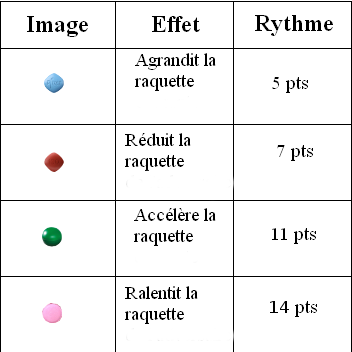
\includegraphics[scale=0.5]{./images/pilules.png}


\subsection{Le réseau}

Le premier joueur est serveur lorsque l'on lance le jeu, cependant la communication se fait dans 
les 2 sens entre les joueurs, serveur et client. Tout d'abord, lorsque le premier joueur lance le jeu, il 
envoie la valeur de son score max au possible client qui se connecterait. Lorsque celui-ci arrive, il 
reçoit le score max et renvoie une chaîne de caractères servant d'accusé de réception (noté ``ack'' dans 
la suite du rapport).
Ensuite, à chaque instant, chacun des joueurs envoie 
la position courante de sa raquette à l'adversaire qui peut ainsi positionner la raquette de son 
adversaire de son point de vue, afin d'être sûr que les 2 applications soient synchronisées. La balle 
est également synchronisée, cependant, pour pouvoir régulièrement vérifier si les valeurs envoyées 
sont les bonnes, les 2 joueurs gèrent la balle à tour de rôle. Lorsque la balle se situe sur la 
première moitié gauche de l'écran, le joueur 1 doit calculer la position et la vitesse de la balle et les envoyer 
au joueur 2 qui peut ainsi récupérer les valeurs et déplacer la balle sur son application à la 
position correspondante, ainsi que lui attribuer la bonne vitesse. Si la balle est sur la moitié droite de l'écran,
c'est ainsi le joueur 
2 qui gère la balle et le joueur 1 qui reçoit les informations, de façon similaire. Les raquettes et la balle 
ont également un système d'ack qui garantit l'envoi des données.
\\
Les données sont envoyées selon un format particulier et suivent le protocole suivant. Une fonction ``send'' 
envoie les données, l'autre joueur les reçoit dans une fonction ``read'' et renvoie un ack qui sera réceptionné 
dans une fonction ``ack''. Si la fonction ``ack'' retourne ``true'', l'envoi et la réception se sont effectués 
correctement, sinon, on renvoie les données. Chacun des trois objets à synchroniser (les raquettes, la balle et 
le score max) le sont à l'aide des fonctions send/read différentes qui seront explicitées plus tard. La fonction ``ack'' 
quant à elle est générique et s'adapte à tous les objets. Voici le format des données qui sont envoyées:

\begin{itemize}
 \item \textit{Coordonnées de la racket: ``x\_racket''double ou ``y\_racket''double}
 \item \textit{Position de la balle: ``x\_ballpos``double ou ''y\_ballpos``double}
 \item \textit{Vitesse de la balle: ''x\_ballspeed``double ou ''y\_ballspeed``double}
 \item \textit{Score max: ''score``int}
\end{itemize}

Ainsi, le nom de l'objet envoyé est un String, et est suivi de la donnée elle-même. La fonction read appelée correspondante 
effectue d'abord la fonction ''readObject`` afin de récupérer le String et vérifie si la valeur récupérée correspond à 
celle attendue. Si tel est le cas, la fonction ''read`` spécifique au type d'objet suivant est appelée et la variable 
à synchroniser est modifiée. Par la suite, la fonction read envoie le message servant d'ack qui est, selon le type de donnée 
envoyé, l'un des suivants:

\begin{itemize}
 \item \textit{Coordonnées de la racket: ``x\_racket\_recu'' ou ``y\_racket\_recu''}
 \item \textit{Ball position: ``x\_ballpos\_recu`` ou ''y\_ballpos\_recu``}
 \item \textit{Ball speed: ''x\_ballspeed\_recu`` ou ''y\_ballspeed\_recu``}
 \item \textit{Score max: ''score\_recu``}
\end{itemize}

L'envoi de chacune des données est contenue dans une boucle ''do while`` de la sorte:

\begin{lstlisting}[language=Java]
do{
	r.send(sock, ballData[0], "x_ballpos");
}while(!r.ack(sock, "x_ballpos_recu"));
do{
	r.send(sock, ballData[0], "y_ballpos");
}while(!r.ack(sock, "y_ballpos_recu"));
do{
	r.send(sock, ballData[1], "x_ballspeed");
}while(!r.ack(sock, "x_ballspeed_recu"));
do{
	r.send(sock, ballData[1], "x_ballspeed");
}while(!r.ack(sock, "x_ballspeed_recu"));
\end{lstlisting}

Ainsi, l'envoi s'est effectué correctement si la chaîne de caractère souhaitée en ack, celle passée en paramètre, 
a été envoyée, la fonction ''ack`` retournant donc ''true``. Sinon, 
on renvoie les données.

\section{Solo}

Nous avons jugé intéressant de ne pas seulement faire un mode multijoueur mais également d'intégrer un mode solo, 
qui donc ne fait forcément pas appel au réseau, auquel nous avons intégré des règles spécifiques.
\\
Pour le lancer, il suffit de sélectionner ''Solo`` dans ''Mode de jeu`` et de lancer la partie à l'aide de ''Play``. 
Les options suivantes ne servent qu'en mode ''Multijoueur``. Le joueur se retrouve face à une raquette, contrôlée par l'IA, 
imbattable. Il est en effet impossible pour lui de marquer un point comme dans le mode multijoueur, car la raquette 
en face calcule la coordonnée y de la balle et se positionne selon elle, lui permettant ainsi de la réceptionner en permanence. 
Le score du joueur est ainsi calculé par le nombre de fois où il arrive à renvoyer la balle. Son score est augmenté de 1 
à chaque rebond et repart à 0 lorsque celui-ci se prend un point. Ce mode solo peut ainsi être vu comme un mode entraînement.

\section{Jeux de tests}

Nos tests sont situés dans la classe Tests.java et on peut les effectuer en lançant le programme avec pour argument 
la chaîne de caractères 
''test``.
Ici, le menu ne se lancera pas mais les tests seront fait automatiquement et l'utilisateur verra s'afficher sur la sortie 
standard le message suivant: ''"Les tests ont été passés avec succès``, si les tests se passent sans problèmes.
Nous avons décidé de créer des tests sur des fonctions jugées fondamentales et complexes, afin d'être sûr que celles-ci 
agissent de la façon attendue, et ce quels que soient les cas. Nous avons ainsi choisi les fonctions ''collision`` et 
''rebound``, situées toutes deux dans la classe ''Pong.java``.
\\
La méthode est similaire pour les 2. Nous lançons un parcours composé de 4 boucles ''for``, la première sélectionnant 
la première puis la deuxième raquette, la deuxième modifiant la trajectoire y de la raquette courante et les 2 suivantes 
bougeant la balle dans l'espace en x et y. Ainsi, nous testons toutes les positions possibles de la balle en fonction de 
toutes les positions possibles de chaque raquette, indépendamment l'une de l'autre. Dans chaque cas, nous vérifions 
si la fonction à tester retourne bien les paramètres attendus. Nous comparons ainsi les résultats dits ''expérimentaux``, 
correspondant aux valeurs réelles, celles obtenues de par les objets ''Pong`` et ''Ball`` créés, avec les résultats 
attendus, c'est-à-dire les valeurs souhaitées dans les fonctions tests.


\chapter{Valorisation du travail réalisé}

Ici, nous allons mettre en valeur notre code en explicitant les différents algortihmes utilisés et notre réflexion 
ayant mené à ce projet final. Pour cela, nous allons notamment voir l'exemple d'un bug que l'on a eu, la façon 
dont on l'a résolu, ainsi que les optimisations ayant permis d'éviter au maximum les redondances dans le code.

\section{Prise en main sur une seule machine}
La première étape du projet a consisté à créer un pong basique sans le réseau. Nous ne sommes
pas parti de rien, le sujet étant 
donné avec du code. Nous avons pu apprendre à nous servir de swing,
l'API de java pour faire une interface,
et commencer la première partie qui a consisté à créer un pong multijoueur, jouable sur une seule machine.
Notre première décision fut de changer l'aspect graphique du jeu, se rapprochant plus du pong originel.
\\
Nous avons repris l'implémentation donnée dans le code de base et le sujet, une 
classe pong qui gère tout le jeu, 
une classe Window qui affiche le rendu et par laquelle l'appel au réseau, contenu dans 
une classe à part, se fera plus tard. Une fonction Main 
lance le jeu et décide ce que feront
le serveur et le client. Enfin, il y a deux classes, Racket et Ball, héritant toutes deux de PongItem, interface 
contenant 3 paramètres 
communs aux 2 objets, ``width'', ``height'' et ``position''.
\\
Le premier problème fut de gérer la collision et le rebond de la balle sur les raquettes. 
Pour cela, nous avons utilisé un algorithme prenant le problème de revers, 
c'est-à-dire que nous avons cherché à savoir si la balle n'était pas sur la 
raquette. En pensant différement, nous avons donc pu contourner le problème.
Le second, le problème lié au rebond, était du à la diférenciation de l'axe x ou l'axe y sur 
lesquels la balle devait rebondir. Avec notre nouveau mode de pensée utilisé et appliqué sur 
le rebond, nous avons pu résoudre ce problème aussi.
Plus tard, dans le projet, nous avons de nouveau modifié le rebond pour avoir quelque chose 
de plus complexe, nous avons coupé la 
raquette en cinq et, selon la partie sur laquelle la balle rebondit, l'orientation de ce dernier et la vitesse 
sera différente.


\section{Passage en réseau}
Une fois le mode de jeu multijoueur mis en place de façon locale, il aura fallu mettre en place le réseau. 
Pour cela, comme expliqué précédement, une classe Réseau a été créée, contenant 2 fonctions, send et read. 
L'envoi et la réception de données et le système d'ack ayant déjà été détaillé, nous allons ici nous concentrer sur le 
mode d'envoi de données choisi, la raison de la multiplicité des fonctions read et send ainsi que celle de l'unicité 
de la fonction ack.
\\
Après la rédaction de plusieurs fonctions send et read, afin d'envoyer et recevoir les données de la racket, de la balle 
et du score max à établir, nous avons réussi à factoriser le tout en obtenant 4 fonctions. Ainsi, les fonctions ``read'' et 
``send'' sont là pour envoyer des coordonnées. Il peut s'agir des coordonnées de position de la racket, de position de la balle 
ou de vitesse de celle-ci. Voici les prototypes de ces 2 fonctions:
\begin{itemize}
 \item \textit{public void send(Socket sock, Point point, String coor)}
 \item \textit{public void read(Socket sock)}
\end{itemize}

Les 2 fonctions prennent ainsi nécessairement la socket pour l'envoi/réception des données. La fonction ``send'', quant à 
elle, prend la variable ``point`` ainsi que le String ''coor`` déterminant l'origine du point ainsi que la 
coordonnée de celui-ci à envoyer.
\\
Les 2 autres fonctions send/read sont les suivantes:
\begin{itemize}
 \item public void sendMaxScore(Socket sock, int scoreMax)
 \item public void readMaxScore(Socket sock)
\end{itemize}

Celles-ci sont appelées une seule fois au début de la partie, contrairement aux 2 précédentes, mais fonctionnent sur le même 
principe, seul le type de donnée diffère. Ici, il s'agit d'un int. Une fonction readMaxScore spécifique a donc été créée afin 
de réceptionner la valeur correctement.
\\
La fonction ack, intégrée dans un do while, comme expliqué précédemment, est générique et s'applique à absoluement tout type 
de donnée, à condition qu'il respecte ces différentes conditions. Tout d'abord, lors du read, la dernière étape 
doit être l'envoi d'une chaîne de caractère unique servant à identifier le type de donnée qui a été réceptionné. Ensuite, 
cette chaîne de caractère doit être passée en paramètre à la fonction ''ack`` qui la comparera avec celle reçue et renverra 
''True`` si se sont les mêmes, ''False`` sinon, entraînant l'envoi de l'information à nouveau. Voici le prototype de 
cette fonction:

\begin{itemize}
 \item public boolean ack(Socket sock, String message)
\end{itemize}

Cette fonction récupère ainsi les informations via la socket et compare la chaîne de caractères obtenue avec la chaîne 
''message`` passée en paramètre.

\section{Extension}

\subsection{Eviter la triche}
Pour éviter la triche, nous avons repris l'algorithme et les explications données dans le sujet. 
On calcule ainsi la position attendue par la balle à l'aide de sa vitesse, puis on 
la compare avec celle reçue. Si ce sont les mêmes, il n'y a pas de triche.
On ajoute l'appel à cet algorithme après les boucles traitant la réception des données.
\\
Plus tard, nous avons ajouté des balles bonus qui augmentent ou diminuent la vitesse. 
Il fallait un signal pour avertir que les raquettes
étaient affectées par les bonus. Grâce à notre implémentation, nous avons un paramètre de type int dans 
la structure racket indiquant si une 
raquette est touchée par un bonus. Il suffit donc de vérifier si cet int était à la bonne valeur pour les deux raquettes.

\subsection{Les balles spéciales et bonus}
La seconde extension que nous avons ajouté fût les bonus. Nous avons commencé par un bonus agrandissant 
la raquette courante du joueur, en prenant en compte le fait qu'il faut gérer une collision différente. 
Il faut donc se servir 
de notre fonction implementée pour les collisions avec en argument
ball et racket. Les bonus étant tous des types de Ball particuliers, ils héritent tous de cette classe. 
\\
Ne voulant pas surcharger le réseau de données, nous avons décidé que chaque jeu gèrera lui-même tous 
les bonus et qu'ils apparaitraient
donc au bout d'un certain nombre de points marqués par les deux joueurs. Ainsi, on garantit 
la synchronisation, le bonus arrivant sur la raquette 
ayant marqué le dernier
point.
\\
Nous avons créé plusieurs données membres pour une classe nomée BallBonusLarger. Tou d'abord, un booléen qui nous 
permet de savoir si le bonus a été créé, qui sert afin de ne pas écrire de données sur des bonus non 
instanciés, grâce à un if.
Puis, un tableau de 2 int, qui correspond au score courant de la partie lors de la création du bonus. Cette donnée 
nous sert à ne pas créer de nouveaux bonus lorsqu'un est déjà instanciée et que le score contenu dans le tableau 
correspond au score où celui-ci a été créé. Cela évite que les bonus apparaissent sans cesse tant que le score n'est pas 
modifié. 
Enfin, un entier qui définit la position Y du bonus, qui correpondra à la hauteur de la dernière balle perdue.
\\
Après cela, nous avons crée de nouveaux bonus. L'un d'entre eux réduit la raquette du joueur qui l'obtient, tandis que 
les autres augmentent sa vitesse ou au contraire, la réduise. 
Pour ce faire, nous avons créé une classe, située au-dessus dans la hiérarchie, nommée 
BallBonus, héritant de Ball. Ainsi, toutes les classes des 
différents bonus héritent de BallBonus. 
Puis, nous avons mis dans cette classe ce que nous avions précédement fait dans 
BallBonusLarger avec un 
constructeur permettant de choisir l'image du bonus. Enfin, nous avons crée des fonctions utilisées lors 
de la création et l'affichage,
utilisant des données membres pouvant être changée par le constructeur, nous permettant de gérer différents paramètres aisément, 
comme le nombre de points à marquer avant que le bonus apparaisse, l'effet que le bonus aura sur la raquette et le sens 
dans lequel il ira. Il se déplacera ainsi sur celui qui a marqué le dernier point s'il s'agit d'un bonus 
considéré comme positif, ou l'adversaire s'il s'agit d'un malus.

\subsection{Menu}
En dernière partie, nous avons décidé d'ajouter un menu qui nous faciliterait, autant à nous, programmeurs, qu'à 
l'utilisateur, 
le lancement d'une partie de pong. Après des recherches pour comprendre la façon dont swing gére les menus, nous 
avons donc créé
une 
classe Menu.
Pour intégrer les données postées par l'utilisateur dans le menu au reste du code, nous 
avons créé des données membres, dans la classe Main, 
accessibles par
toutes les classes permettant de gérer les différentes options du menu. 
Nous avons aussi créé un thread, que nous avons utilisé 
dans le Main, pour attendre que l'utilisateur lance le jeu avant de commencer à lancer le réseau, puisqu'il nous 
fallait les réponses de celui-ci.
Une des options du menu en début de partie est le score max que doit atteindre un joueur pour gagner une partie, et donc il 
fallait aussi gérer les joueurs qui ne mettraient pas la même valeur, alors qu'ils jouent ensemble. Pour contourner 
ce problème, 
nous avons décidé que ce serait le serveur qui choisirait le score max et qui l'enverrait en début de partie au client.
Enfin, nous avons créé une boîte de dialogue pour la fin d'une partie, lancée lorsqu'un joueur atteint le score maximum et 
proposant deux options: une permettant de rejouer, l'autre de fermer la fenêtre du jeu. La seule chose 
à réinitialiser pour une nouvelle partie
fût le score, et pour la fermeture de la fenêtre, on envoie un entier qui nous permet de sortir 
de la boucle while de Window, 
là où toute la partie affichage se fait.
\chapter{Diagramme des classes}

%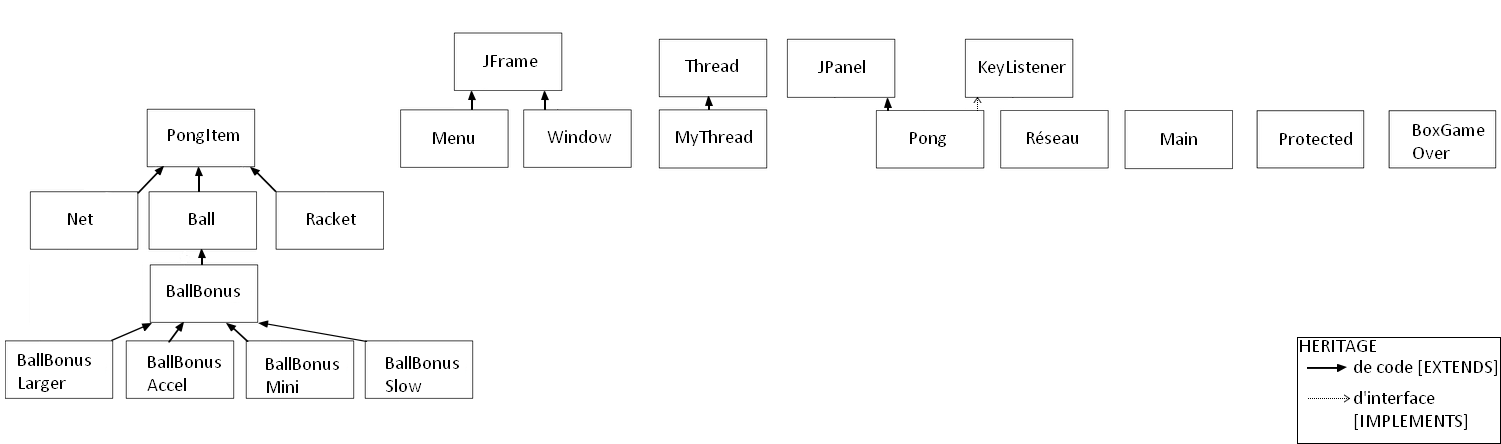
\includegraphics[scale=0.5]{./images/diagramme}

\begin{figure}[h]
 \hspace*{-3.5cm}
 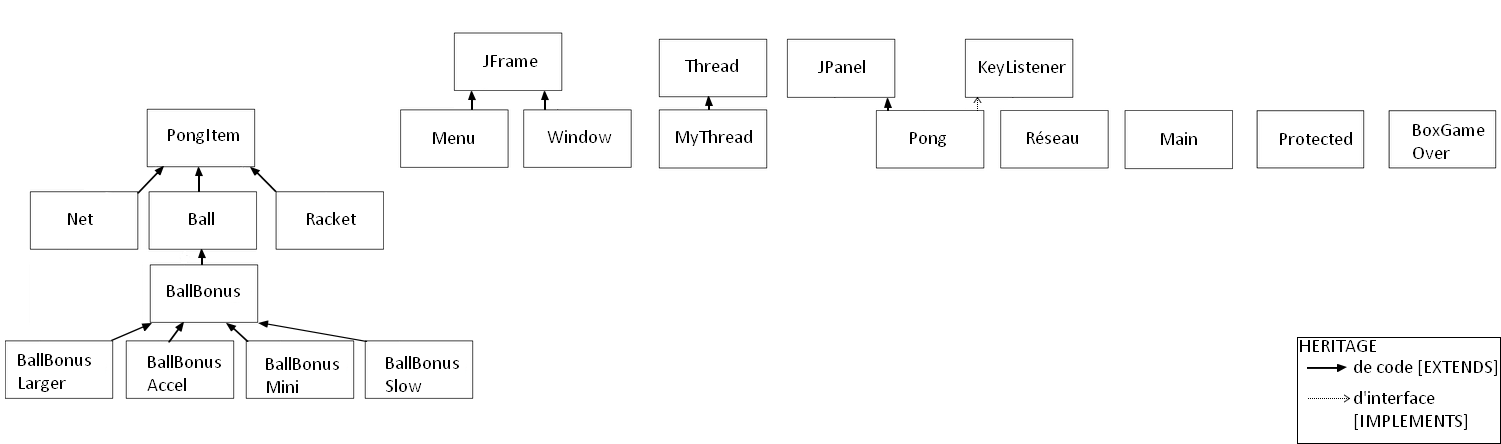
\includegraphics[scale=0.5]{./images/diagramme}
\end{figure}
\chapter{Conclusion}

Le bilan de ce projet est globalement positif. Nous pensons avoir réussi, de manière efficace, à mettre en place 
un pong en réseau, le tout en lui ajoutant de nombreux élèments facultatifs, tels que la mise en place du menu, 
le mode solo ou les balles bonus.
\\
Cependant, lors de la création de celui-ci, nous avions eu de nombreuses idées d'implémentations supplémentaires qui n'ont 
pas été ajoutées, faute de temps et par volonté de se concentrer sur des aspects plus fondamentaux.
Parmi ces fonctionnalités, il y a la possibilité de jouer à quatre joueurs 
simultanément. Il aurait donc fallu modifier notre réseau pour que toutes les machines se connectent entre elles 
et soient à la fois serveur et client. Dès lors qu'une machine se connecterait à une autre, celle-ci lui enverrait 
les noms des 
autres machines auxquelles il faudrait se connecter. On aurait donc pu gérer la balle non plus sur deux machines, 
mais sur quatre, 

et il aurait fallu modifier le code du jeu en rajoutant deux raquettes, en haut et en bas, avec un score différent pour
chacun. Nous aurions aussi aimé pouvoir griser les menus lorsque ceux-ci sont inutiles, par exemple, lorsque l'on est 
serveur, l'option demandant l'adresse ip est inutile, nous aurions donc voulu que le menu soit dynamique et change
dès que l'on 
choisit une option. Cependant, nous avons évidemment adapté l'implémentation, de façon à ce que, si un joueur étant serveur
tape une adresse IP ou que le client souhaite déterminer le score à atteindre lui-même, ces valeurs ne soient pas prises 
en compte. Enfin, d'autres idées de bonus nous ont plu et seront probablement implémentées à l'issue de ce projet, comme 
le fait de jouer avec plusieurs balles, obtenir une raquette aimantée bloquant la balle quelques secondes, un malus 
inversant les touches, un bonus offrant une possibilité de mouvement selon l'axe x temporairement etc..
\\
Enfin, nous ne garantissons pas aux joueurs une protection face à tout type de triche, et ce malgré notre algorithme, 
même s'il paraît bien sûr impossible de faire cela. Nous pensons malgré tout que celui-ci peut-être 
améliorable, bien que nous considérons néanmoins qu'il offre au joueur une garantie correcte au vu de l'ampleur du projet.
\chapter{Bibliographie}
Voici les différents supports nous ayant aidé pendant le développement du projet. Il s'agit de sites web, ainsi, ceux-ci 
peuvent avoir été modifiés depuis leur consultation, pendant la durée du projet.
\\ 
\\ 
\\
\textit{Cours par M. Cyrille HERBY pour l'utilisation de swing:} https://openclassrooms.com/courses/apprenez-a-programmer-en-java/les-menus-et-boites-de-dialogue
\\
\\
\textit{Documentation Java Oracle pour diverses informations sur les fonctions (notamment pour la classe réseau):} https://docs.oracle.com/javase/7/docs/api/
\\
\\
\textit{Support de cours de M. Samuel THIBAULT}: http://dept-info.labri.fr/~thibault/Reseau/support.pdf

\chapter{Annexes et code du projet}
Cette annexe aura pour objectif de présenter l'ensemble des documents liés au projet, à commencer par le sujet.

\end{document}
